\documentclass[german,12pt,a4paper,oneside]{report}
\usepackage{hyperref} %sorgt f�r links im erzeugten pdf
\usepackage[ngerman]{babel}
\usepackage{listings} %wird f�r code listings verwendet
\usepackage{color}
\usepackage{pdfpages} %wird f�r includepdf verwendet
\usepackage{graphicx} %wird f�r includeimage verwendet
%\usepackage[xindy,toc]{glossaries}
\usepackage[T1]{fontenc} %damit sonderzeichen wie | richtig angezeigt werden
\usepackage[latin1]{inputenc} %damit Umlaute verwendet werden k�nnen
\usepackage{fancyhdr} %Packet f�r fany headers
\usepackage{todonotes} %Packet f�r TODOs
\usepackage{setspace} %f�r Zeilenabstand
\usepackage{sectsty} %damit der Abstand der �berschriften ver�ndert werden kann
\usepackage{datetime} %f�r \monthname{}
\definecolor{dkgreen}{rgb}{0,0.6,0}
\definecolor{gray}{rgb}{0.5,0.5,0.5}
\definecolor{mauve}{rgb}{0.58,0,0.82}
 
\lstset{ %
  language=VHDL,                  % the language of the code
  basicstyle=\footnotesize,       % the size of the fonts that are used for the code
  numbers=left,                   % where to put the line-numbers
  numberstyle=\tiny\color{gray},  % the style that is used for the line-numbers
  stepnumber=1,                   % the step between two line-numbers. If it's 1, each line will be numbered
  numbersep=5pt,                  % how far the line-numbers are from the code
  backgroundcolor=\color{white},  % choose the background color. You must add \usepackage{color}
  showspaces=false,               % show spaces adding particular underscores
  showstringspaces=false,         % underline spaces within strings
  showtabs=false,                 % show tabs within strings adding particular underscores
  frame=single,                   % adds a frame around the code
  framexleftmargin=5mm,           % margin adujsted to that line-numer is inside of the frame
  rulecolor=\color{black},        % if not set, the frame-color may be changed on line-breaks within not-black text (e.g. commens (green here))
  tabsize=2,                      % sets default tabsize to 2 spaces
  captionpos=b,                   % sets the caption-position to bottom
  breaklines=true,                % sets automatic line breaking
  breakatwhitespace=false,        % sets if automatic breaks should only happen at whitespace
  title=\lstname,                 % show the filename of files included with \lstinputlisting;
                                  % also try caption instead of title
  keywordstyle=\color{blue},      % keyword style
  commentstyle=\color{dkgreen},   % comment style
  stringstyle=\color{mauve}%,      % string literal style
%  escapeinside={\%*}{*)},         % if you want to add a comment within your code
%  morekeywords={*,...}            % if you want to add more keywords to the set
}

\onehalfspacing %1.5 Zeilen Abstand
\addtolength{\parskip}{\baselineskip} %Macht den Abstand eines Absatzes genau eine Zeile gro�.
\setlength\parindent{0pt} %Schaltet das automatische Einr�cken f�r einen neuen Absatz aus
%\selectlanguage{\german} %deutsch als Sprache f�r �berschriften
%\pagestyle{headings} %Kapitel�berschrift und Seitenzahl in der Kopfzeile
%\pagestyle{fancy} %fancy header and footer

%�berschrift nach links schieben
\sectionfont{\hspace{-1 cm}}
\subsectionfont{\hspace{-1 cm}}
%\subsubsectionfont{\hspace{-1 cm}}

%plain wird neu definiert, damit es auch bei chapter funktionert, da diese default m��ig \pagestyle{plain} verwenden
\fancypagestyle{plain}{%
\fancyhead{}
\fancyfoot{}
\fancyhead[L]{\leftmark}
\fancyhead[R]{\thepage}
\setlength{\headheight}{15pt}
\renewcommand{\headrulewidth}{0.4pt} %obere Trennlinie
%\renewcommand{\footrulewidth}{0.4pt} %untere Trennlinie
}

\pagestyle{plain}
%default format \renewcommand{\chaptermark}[1]{\markboth{\MakeUppercase{\chaptername\ \thechapter.\ #1}}{}}
\renewcommand{\chaptermark}[1]{\markboth{\textit{#1}}{}} %format vom text im header 
\newcommand{\myaddcontentsline}[3]{\begin{singlespace} \addcontentsline{#1}{#2}{\vspace{-2ex} #3} \end{singlespace}} %\addcontentsline{toc}{chapter}{Lebenslauf}

\renewcommand{\lstlistlistingname}{Quellcodeverzeichnis}
\renewcommand{\lstlistingname}{Quellcode}
%\includeonly{chapter3}
\begin{document}
\includepdf{deckblatt/coversheet} %Titelblatt einf�gen
\setcounter{page}{1} %Beginne wieder bei 1 zu z�hlen

\renewcommand{\thepage}{\Roman{page}} %gro�e r�mische Zahlen
\selectlanguage{english}
\chapter*{Abstract}
\markright{Abstract}
VHDL is a strongly typed language that is used for modelling digital circuits such as CPUs, GPUs and
others, and is besides Verilog the most spread.

As for many other tools in the Electronic Design Automation (EDA) industrie, there are no modern open source compiler and other tools available. With GHDL exists a compiler, but it is based on GCC and is written in Ada, with all thereby following disadvanteges. 

As more and more languages are implemented ontop of the Java Virtual Machine (JVM), this machine was also used as a target because of the later explained adavantages. This work presents the desing and implementation of this compilers which can compile a subset of VHDL into JVM Byte code.

\selectlanguage{ngerman}
\chapter*{Kurzfassung}
\markright{Kurzfassung}
VHDL ist eine stark typisierte Sprache die zur Modellierung von digitalen Schaltungen wie CPUs, GPUs und
anderer verwendet wird, und ist neben Verilog die am st�rksten verbreitetste.

Wie f�r viele andere Tools in der Electronic Design Automation (EDA) Industrie, sind f�r VHDL keine modernen Open Source Compiler und andere Tools vorhanden. Mit GHDL gibt es zwar einen Compiler, der aber auf GCC aufsetzt und in Ada geschrieben ist, mit allen den damit folgenden Nachteilen. 

Da mehr und mehr Sprachen auf der Java Virtual Machine (JVM) implementiert wurden, wurde diese auch als Ziel verwendet aufgrund der sp�ter erl�utertenden Vorteile. Diese Arbeit pr�sentiert das Design und die Implementierung dieses Compilers der eine Teilmenge von VHDL in JVM Byte Code �bersetzen kann.

%\setcounter{tocdepth}{3} %Inhaltsverzeichniss bis zur Tiefe 3 rendern
\singlespacing
\tableofcontents %Inhaltsverzeichniss
\chaptermark{Inhaltsverzeichniss}
\newpage
\setcounter{page}{1} %Beginne wieder bei 1 zu z�hlen
\renewcommand{\thepage}{\arabic{page}} %arabische Zahlen
\onehalfspacing
\chapter{Aufgabenstellung und Motivation}
{\em 
Diese Kapitel gibt einen kurzen �berblick �ber die Aufgabenstellung und die Motivation der Masterarbeit.
Zus�tzlich wird wird eine �bersicht �ber die verschiedenen Themen die in den einzelnen Kaptitel beschrieben werden, gegeben.
}

Die in VHDL beschriebenen Schaltungen m�ssen vor der Logiksynthese am Computer simuliert werden, um sie auf m�gliche Fehler zu �berpr�fen. Die dazu ben�tigten Software-Werkzeuge sind bis auf eine Ausnahme nur von kommerziellen Anbietern erh�ltlich und f�r Studenten gar nicht oder nur f�r in der Gr��e beschr�nkte Schaltungen erh�ltlich.

Diese Einschr�nkungen waren die Motivation dieser Arbeit und das Ziel dieser ist es, einen Compiler f�r einen ausreichend gro�en Teilbereich des VHDL 2002 Standards zu implementieren, um damit reale Chip-Designs erfolgreich simulieren zu k�nnen.

Folgende Probleme sind dabei zu l�sen:
\begin{itemize}
\item Es muss ein Parser erstellt werden und es soll darin durch semantische Aktionen ein Abstrakter Syntaxbaum erzeugt werden, der in weiteren Verarbeitungsschritten manipuliert werden kann.
\item Im n�chsten Schritt muss der erzeugte AST traversiert werden um die Symboltabelle zu verwalten damit die n�tigen Typ�berpr�fungen durchgef�hrt werden k�nnen. Es soll auch darauf geachtet werden, dass f�r den Benutzer des Compilers gute und hilfreiche Fehlermeldungen erzeugt werden.
\item Anschlie�end muss der erzeugte Zwischencode in JVM-Bytecode �bersetzt werden. Dabei ist zu beachten, dass die Semantik der Sprache nicht verloren geht und wie eventuelle Beschr�nkungen der JVM zu umgehen sind (z.B out Parameter).
\end{itemize}

\section{Aufbau}
Diese Masterabeit ist wie folgt aufgebaut:
\begin{itemize}
	\item In Kapitel 2 wird eine Einf�hrung in VHDL gegeben.
	\item Kapitel 3 er�rtert die Architektur des Compilers
	\item Kapitel 4 wird der gew�hlte Ansatz mit anderen Compilern verglichen
	\item Kapitel 5 fasst die Arbeit zusammen und gibt einen Ausblick auf weitere m�gliche Verbesserungen
\end{itemize}

\chapter{VHDL}
{\em 
In diese Kapitel wird ein �berblick �ber die Sprache VHDL geben. Zuerst wird die Geschichte und Standards erl�utert, anschlie�end die Sprache selbst.
}
\section{Geschichte}
VHDL (Very High Speed Integrated Circuit Hardware Description Language oder auch VHSIC Hardware Description Language) ist eine vom IEEE standardisierte Sprache zur Beschreibung digitaler Schaltungen, die von Hardware Designern f�r aktuelle Designs verwendet wird.

VDHL ist neben Verilog eine der weltweit am meisten genutzten Hardwarebeschreibungssprachen und hat sich in Europa zum "Quasi-Standard" entwickelt. Die erste Spezifikation der Sprache wurde in den fr�hen 1980er Jahren entwickelt und ist das Ergebnis von Normierungsbestrebungen eines Komitees, in dem die meisten gr��eren CAD-Anbieter und CAD-Nutzer, aber auch Vereinigungen wie die IEEE, vertreten waren. Der gr��te nordamerikanische Anwender, das US-Verteidigungsministerium, hat VHDL zum Durchbruch verholfen, indem es die Einhaltung der Syntax von VHDL als notwendige Voraussetzung f�r die Erteilung von Auftr�gen gemacht hat. \cite{ash}

VHDL was originally developed at the behest of the U.S Department of Defense in order to document the behavior of the ASICs that supplier companies were including in equipment. That is to say, VHDL was developed as an alternative to huge, complex manuals which were subject to implementation-specific details.

The idea of being able to simulate this documentation was so obviously attractive that logic simulators were developed that could read the VHDL files. The next step was the development of logic synthesis tools that read the VHDL, and output a definition of the physical implementation of the circuit.

Due to the Department of Defense requiring as much of the syntax as possible to be based on Ada, in order to avoid re-inventing concepts that had already been thoroughly tested in the development of Ada,[citation needed] VHDL borrows heavily from the Ada programming language in both concepts and syntax.

\subsection{Versionen und Standards}
Die Initiale Version von VHDL wurde unter dem IEEE Standard 1076-1987 ver�ffentlicht, und enthielt verschiedene Datentypen, numerische (integer and real), logische (bit and boolean), character und time, und arrays von bit und character (bit\_vector string)

Danach wurde erkannt, dass sich mit den vorhanden Datentypen "multi-valued logic" wo ein Signal mehrere Zust�nde (undefiniert, schwach, stark) nicht modellieren lassen kann. Dieses Problem wurde mit dem IEEE 1164 Standard gel�st, der die zus�tzlichen 9-wertige logische Datentypen scalar std\_ulogic und std\_ulogic\_vector definiert.

Im Jahr 1993 wurde eine Aktualisierung des Standards ver�ffentlicht, der die Syntax konsistenter machte, den Zeichensatz auf ISO-8859-1 erweiterte und den XNOR Operator einf�hrte.

Kleiner �nderungen des Standards im Jahr 2002 und 2002 f�gten VHDL unter anderem die schon den in Ada bekannten protected types hinzu, mit dem sich wechselseite Ausschl�sse definieren lassen k�nnen.

Neben dem IEEE Standard 1076, der die eigentliche Sprache definiert, gibt es zus�tzlich noch verwandte die Sprache erweitern oder Funktionalit�t von verschiedenen Libraries beschreibt. Der Standard 1076.2 f�gt mehr added better handling of real and complex data types, 1076.3 f�hrt signed und unsigned Datentypen ein, mit denen arithmetische Operationen auf arrays ausgef�hrt werden k�nnen. IEEE Standard 1076.1 (besser bekannt als VHDL-AMS) beschreibt Erweiterungen f�r gemischte analog und digitale Schaltungen.

Im Juni 2006, wurde durch eine technisches Komittee ein Enwurf f�r VHDL-2006 vorgelegt. Dieser Entwurf war vollkommen abw�rtskompatibel mit �lteren Versionen, f�gte aber viele Erweiterungen hinzu die das Schreiben von Code erleichterten. Die wichtigste �nderung war, dass die verwandten Standards 1164, 1076.2, 1076.3 in den 1076 Standard hinzugef�gt wurden. Zus�tzlich wurden neue Operatoren , flexiblere Syntax f�r case und generate Statements und es wurde ein Interface zu C/C++ hinzugef�gt.

Im Jahr 2008 wurde eine neuere Version dieses Entwurf, nachdem die bisher darin entdecken Probleme gel�st wurden, ver�ffentlicht. Anschlie�en wurde die letzte Version als IEEE 1076-2008 Standard im Januar 2009 ver�ffentlicht.
\section{Sprachumfang}
\lstset{caption={Beispiel f�r ein AND Gate},label=ANDGATE}
\lstinputlisting{src/ANDGATE.vhd}
\chapter{Architektur des OpenVC Compilers}
{\em 
In diese Kapitel wird die Architektur erl�utert, dynamische sowie statische. Es wird dabei erkl�rt wie VHDL Source Code durch den OpenVC Compiler verarbeitet wird.
}
\section{Statische und dynamiche Architektur}
\subsection{Phasen}
Der Compiler verarbeitet den Source Code in vier verschiedenen Phasen
\begin{figure}
  \centering
    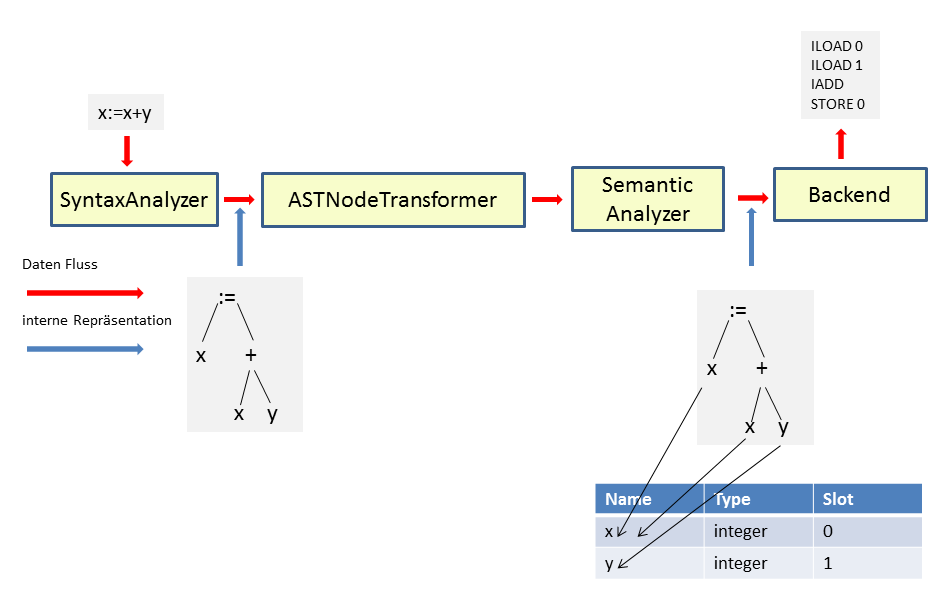
\includegraphics[scale=0.7]{images/CompilerPhasen.png}
    \caption{Die vier Phasen des Compiler}
\end{figure}

\subsection{Klassen�bersicht}
\todo{Text}
\section{Scanner/Parser mit Antlr}
\begin{quotation}
Eine Grammatik hei�t LL(1) (d.h. analysierbar von links nach rechts mit linkskanonischen Ableitungen und einem Vorgriffssymbol), wenn an jeder Stelle, an der man zwischen mehreren Alternativen w�hlen kann, gilt, dass die terminalen Anf�nge dieser Alternativen paarweise disjunkt sind. Mit anderen Worten: Der Parser muss jederzeit mit einem einzigen Vorgriffssymbol entscheiden k�nnen, welche von mehreren m�glichen Alternativen er w�hlen soll. \cite{moess}
\end{quotation}

Die im Standard \cite{ieee} beschriebene Syntax liegt bereits in Extended Backus-Naur Form (EBNF) \cite{wirth} vor, weist aber einige LL(1) Konflikte auf, die vorher behoben wurden.
In der Beschreibung von Coco/R [M�ss03] werden drei verschiedene M�glichkeiten erl�utert, wie diese Konflikte gel�st werden k�nnen. Mit Hilfe dieser drei Varianten ist es auch gelungen, die Grammatik in eine f�r Antlr valide LL(1) Form umzuwandeln. Die drei Ans�tze zur Behebung der Konflikte werden nachstehend erl�utert.

\subsection{Faktorisierung}
Bei der Faktorisierung werden gemeinsame Teile herausgezogen und an den Anfang der Produktion gestellt. Z.B. kann die folgende Produktion
\begin{center} A = a b c | a b d. \end{center} 
in die Produktion A'
\begin{center} A' = a b (c | d). \end{center} 
ohne Konflikte umgewandelt werden.
\todo{Beispiel}
%\lstset{caption={}}
%\lstinputlisting[style=ANTLR]{src/test.g}

\subsection{Umwandlung in Iterationen}
Linksrekursion stellt in LL(k) Sprachen im Gegensatz zu LR basierten immer ein Problem dar. In der Produktion
\begin{center} A = A b | c. \end{center} 
starten beide Alternativen mit c. Durch eine Umwandlung der Rekursion in eine Iteration kann dieses Problem gel�st werden, z.B wird die Produktion A zu
\begin{center} A' = c \{b\}. \end{center}
\todo{Beispiel}
\subsection{Einsatz von \textit{Conflict Resolvers}}
Bei dem Einsatz von \textit{Conflict Resolvers} kann unterschieden werden, wie viele Tokens der Parser vorausschauen muss, um eine Entscheidung zu treffen.

\subsubsection{Konstante Anzahl von \textit{Lookahead Tokens}}
Diese F�lle k�nnten meistens auch durch den Einsatz von Faktorisierung gel�st werden, aber die Lesbarkeit der Grammatik w�rde darunter leiden. Durch die Ber�cksichtigung von mehreren Tokens in die Entscheidung verh�lt sich der Parser effektiv wie ein LL(k) basierter.
\todo{Beispiel}

\subsubsection{Unbekannte Anzahl von \textit{Lookahead Tokens}}
Hier muss der Parser beliebig viele Tokens konsumieren und wird dabei in einen LL(*) basierten umgewandelt. [Par07]
\todo{Beispiel}

\section{AST}
\subsection{AST Konstruktion}
\todo{Text}

\subsection{AST Beispiel}
Im folgenden Abschnitt wird anhand von konkreten Beispielen genauer verdeutlich, wie der konstruierte AST im Speicher dargestellt wird, wobei die einzelnen Kanten der Graphen die Variablen der verschiedenen Klassen darstellen. Es wird zuerst immer der entsprechende Programmcode gezeigt und anschlie�end der entsprechende Graph mit den AST-Knoten.

\subsubsection{WhileStatement}
\lstset{caption={},language=VHDL}
\lstinputlisting{src/WhileStatement.vhd}
\begin{figure}
  \centering
    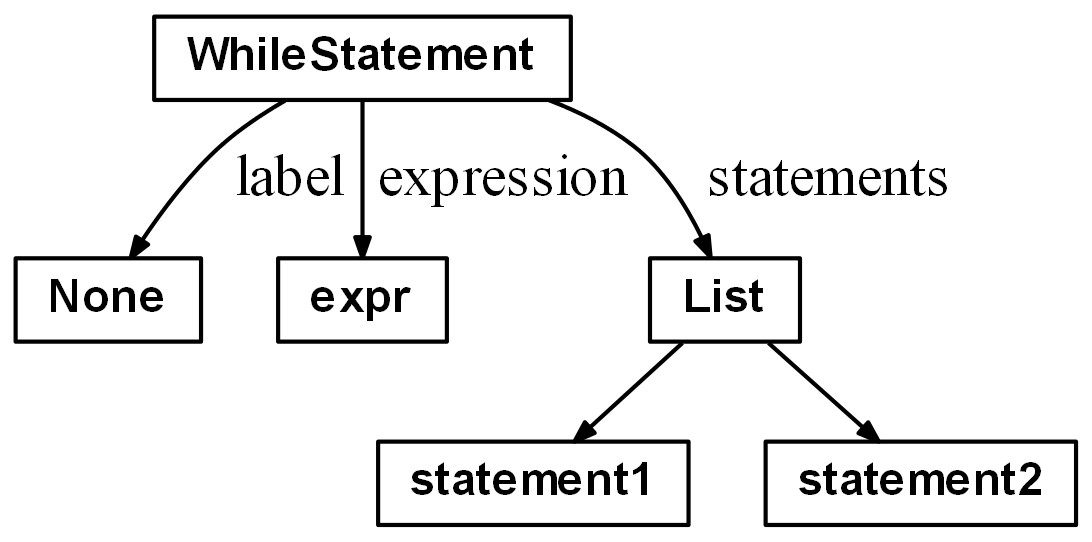
\includegraphics[scale=0.6]{images/WhileStatement.png}
    \caption{AST-Knoten f�r ein While-Statement}
\end{figure}
Ein While-Statement besteht aus einer Expression, die in der Variable \textit{expression} gespeichert wird und einer Liste von Statements die in \textit{statements} gespeichert werden.

\subsubsection{IfStatement}
\lstset{caption={}}
\lstinputlisting{src/IfStatement.vhd}
\begin{figure}
  \centering
    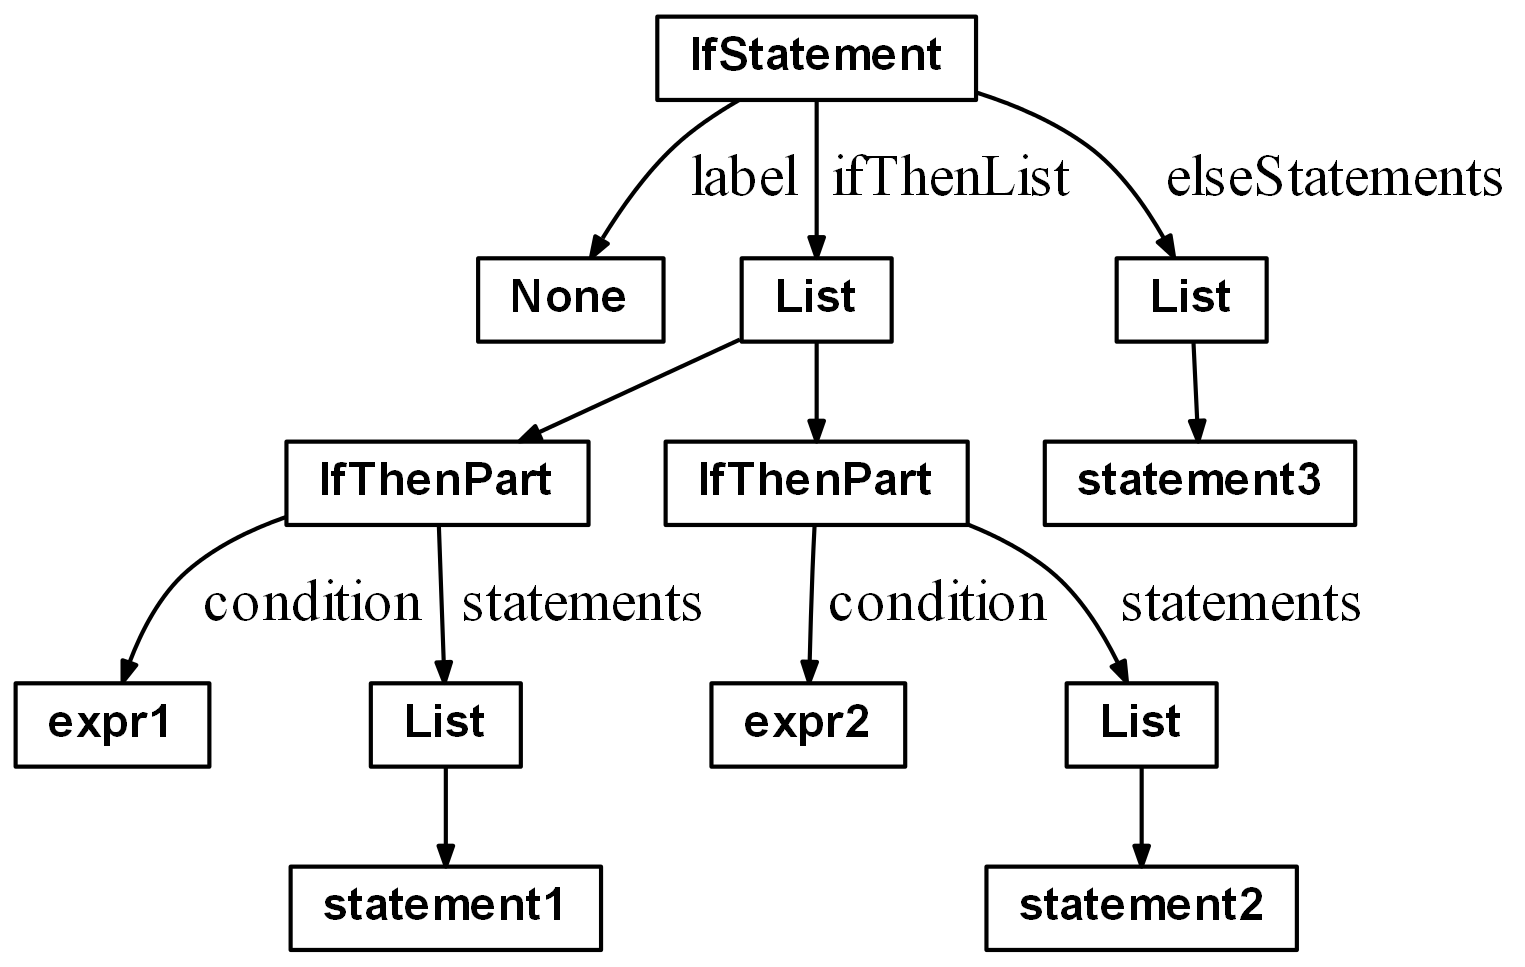
\includegraphics[scale=0.6]{images/IfStatement.png}
    \caption{AST-Knoten f�r ein While-Statement}
\end{figure}
Ein If-Statement besteht aus mehreren Zweigen, wobei die einzelnen Zweige Instanzen der Klasse IfThenPart sind, wo die Condition und die Liste der Statements gespeichert werden. Die Variable elseStatements enth�lt die Statements aus dem else-Zweig.

\subsubsection{LogicalExpression}
\lstset{caption={}}
\lstinputlisting{src/LogicalExpression.vhd}
\begin{figure}
  \centering
    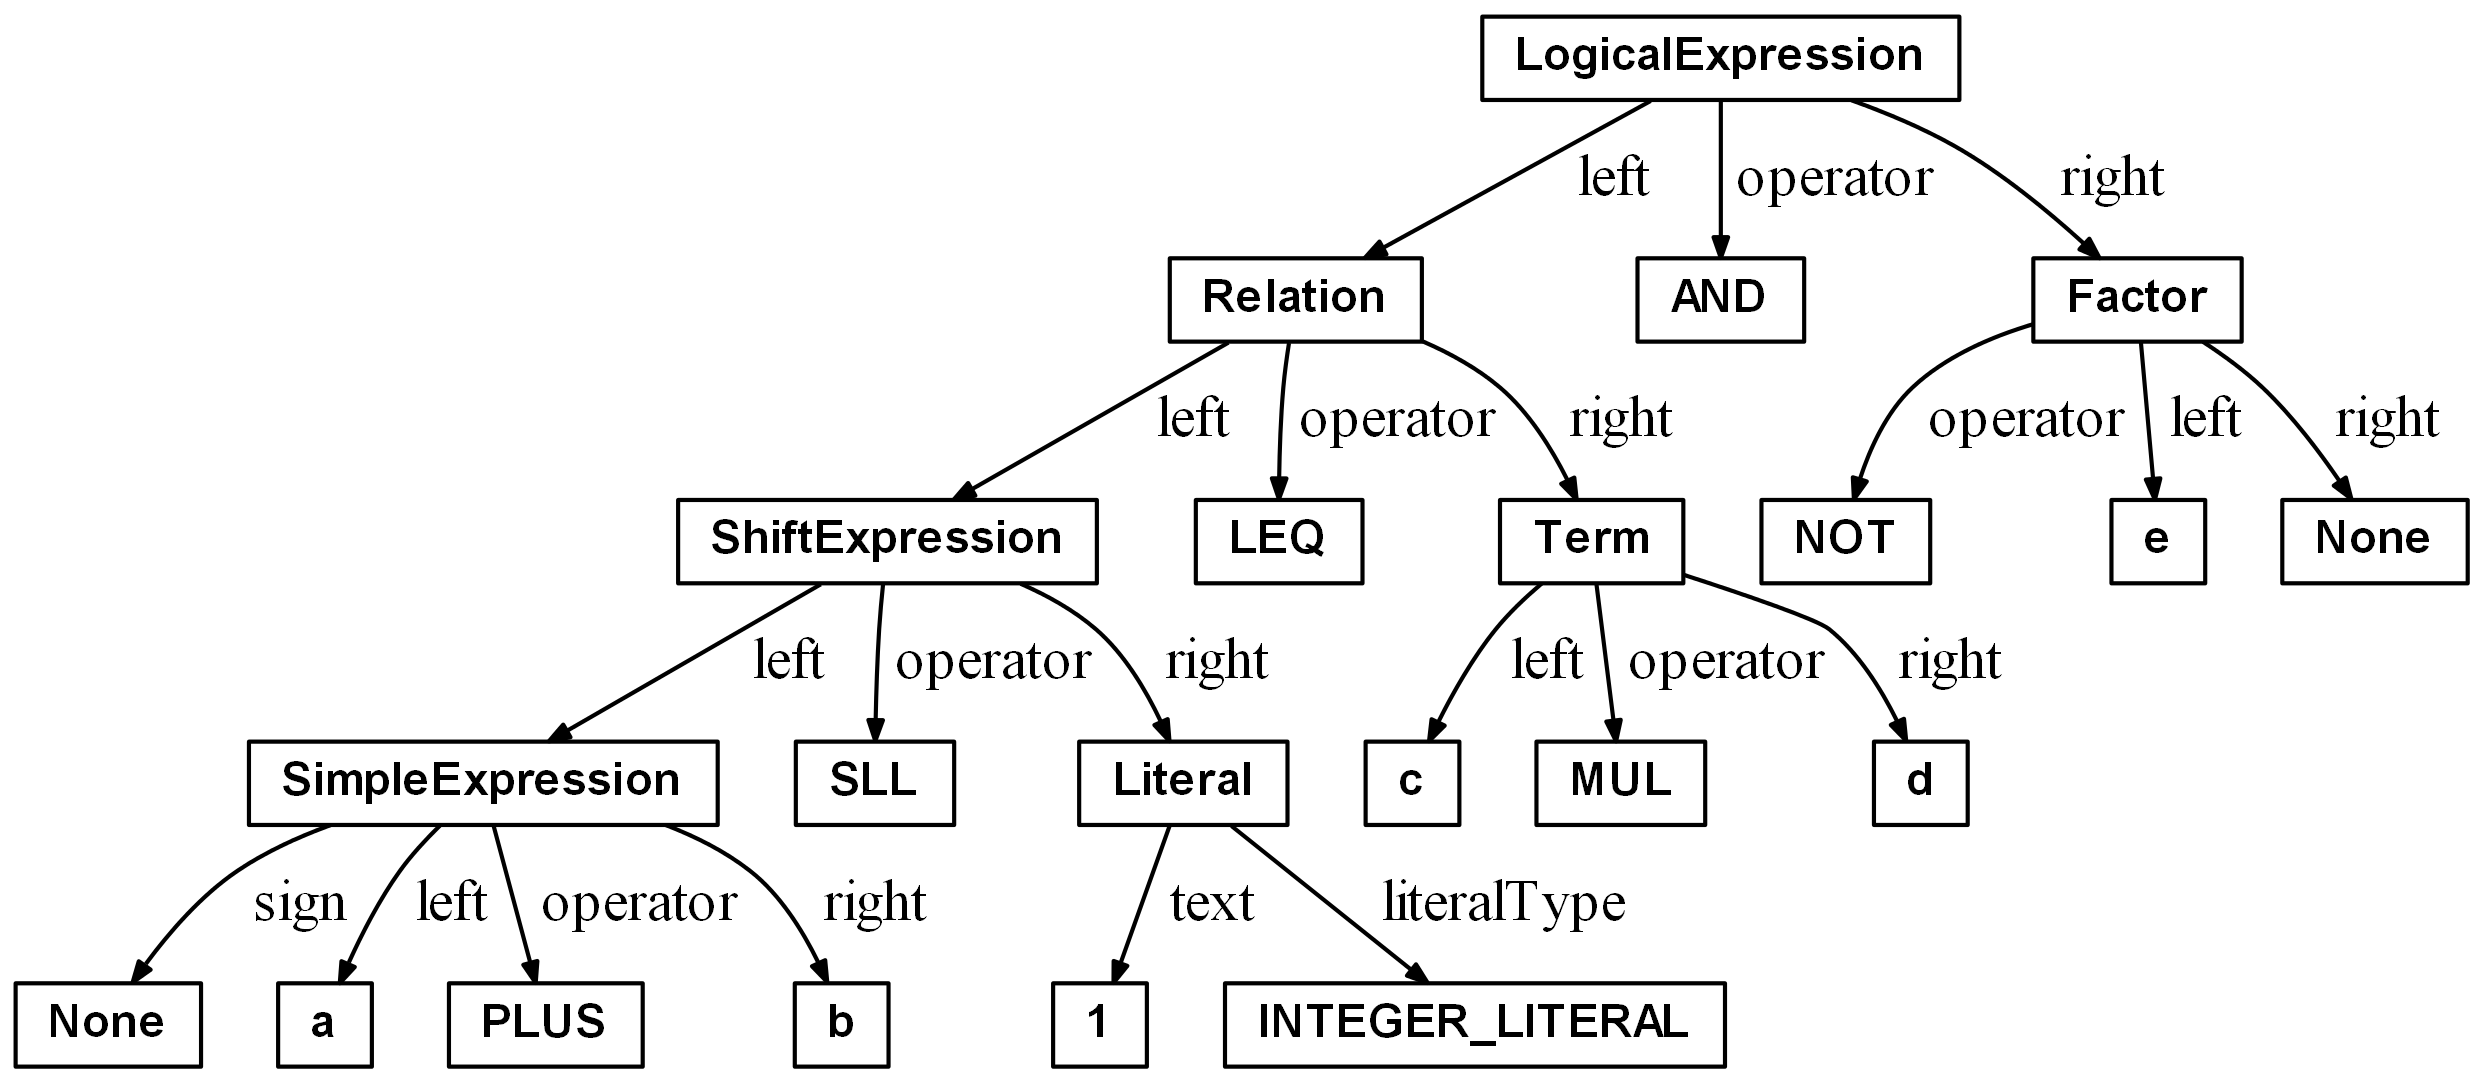
\includegraphics[scale=0.6]{images/LogicalExpression.png}
    \caption{AST-Knoten f�r eine Logical-Expression}
\end{figure}
Eine Logical-Expression besteht wie alle Binary-Expression aus einer linken und rechten Expression und einem Operator der beide miteinader verkn�pft.

\subsubsection{ConstantDeclaration}
\lstset{caption={}}
\lstinputlisting{src/ConstantDeclaration.vhd}
\begin{figure}
  \centering
    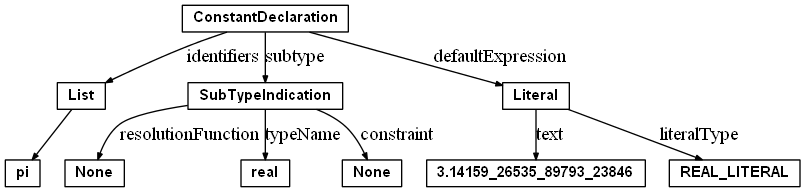
\includegraphics[scale=0.6]{images/ConstantDeclaration.png}
    \caption{AST Knoten f�r eine Constant-Declaration}
\end{figure}
Die Deklaration f�r eine Konstante besteht aus einer Liste von Identifiers, einer Type Beschreibung und einem Default-Wert.

\subsection{AST Manipulation}
\todo{Text}
\section{Symboltabelle}
\section{Codeerzeugung}
%%\chapter{Semantische Analyse}
\chapter{Codeerzeugung}
In der letzten Phase, dem \textit{Backend}, wird der komplete AST noch einmal rekursiv traversiert um als Ergebnis des �bersetzungsvorgangs JVM-Byte Code zu erzeugen.
In diesem Kapitel wird der Einfachheit halber nicht direkt der erzeugte Byte Code besprochen, sondern es wird VHDL-Code mit Java Code verglichen. Dieser ist
�quivalent zum tats�chlich produzierten Byte Code l�sst sich aber leichter erkl�ren.
Auch wird hier die Umwandlung aus Platzgr�nden nur f�r ausgew�hlte Aspekte und VHDL-Konstrukte erl�utert, die interessant oder repr�sentativ f�r die restlichen sind.

Die eigentliche Codeerzeugung wurde mit der Hilfe der ASM Library \cite{ASM} implementiert. 
ASM nimmt dem Entwickler viele Details ab, wie das Verwalten des Konstantenpools, und bietet mit seiner API ein abstrahiertes Modell der JVM.

Im nachfolgenden Code werden teilweise Namen mit einem \$-Zeichen gezeigt. Der Grund liegt darin, dass \$ kein valides Zeichen f�r VHDL Bezeichner ist, aber die JVM akzeptiert diese.
Durch die Verwendung von \$ kann es zu keinen Namens-Konflikten f�r zus�tzlich vom Compiler erzeugte Variablen und Methoden kommen. 

\section{VHDL-Packages}
\subsection{Package Header}

\todo{text}
\lstset{caption={\textit{Package Header}}, label=package_vhdl, numbers=left, language=VHDL}
\lstinputlisting{src/backend/package.vhd}

\lstset{caption={Generierter Code}, label=package_java, language=Java}
\lstinputlisting{src/backend/package.java}
\subsubsection*{\textit{Name Mangling}}
Die etwas kryptisch erscheinenden Namen der generierten Funktionen sind n�tig, da beide Funktionen die gleiche JVM Signature aufweisen. \textit{IntA} und \textit{IntB} sind zwar in VHDL unterschiedliche Typen, aber f�r beide wird der gleiche Code produziert.
Diese Umbennenung wird durch das \textit{name mangling} durchgef�hrt. Dazu wird zum urspr�nglichen Namen der Hash-Wert aus den Namen und Typen aller Parameter der Prozedur angeh�ngt.

\subsubsection*{\textit{Standardwerte}}
Auch wird hier die Behandlung von Standardwerten ersichtlich. Die beiden Funktionen \textit{\$default\$proc\$1636619\_x} und \textit{\$default\$proc\$4355160\_x} werden erzeugt und liefern nur den Standardwert f�r \textit{x} in den zwei \textit{proc} Prozeduren zur�ck.
Standardwerte k�nnen beliebige Ausdr�cke sein, die unterschiedliche Werte ergben und werden daher jedesmal neu ausgewertet. Daher reichen Konstanten nicht und es m�ssen Methoden verwendet werden.

\subsection{\textit{Package Body}}
\begin{minipage}{.48\textwidth}
	\lstset{caption={\textit{Package Body}-Deklaration}, label=package_body_vhdl, numbers=left, language=VHDL}
	\lstinputlisting{src/backend/package_body.vhd}
\end{minipage}
\hfill
\begin{minipage}{.48\textwidth}
	\lstset{caption={Erzeugter Code f�r \textit{Package Body}}, label=package_body_java, language=Java}
	\lstinputlisting{src/backend/package_body.java}
\end{minipage}
Nachdem die Schnittstellen im \textit{header} festgelegt sind, werden die Funktionen im \textit{body} definiert. Dabei entsteht aus dem \textit{package} \textit{p} die Klasse \textit{p\_body} mit nur statischen Methoden, da es nur eine Instanz des \textit{body} gibt.
Hierbei ist wieder das name-mangling durch den Compiler ersichtlich.

\section{Statements}
Im Anschlu� werden einige Statements n�her erl�utert. 
Alle weiteren wie \textit{While}-, \textit{Procedure-Call-}, \textit{Case} und \textit{If}-Statement k�nnen meistens leicht eins zu eins �bersetzt werden und werden daher auch nicht n�her erkl�rt.

\subsection{Schleifen}
\subsubsection{\textit{For}-Schleife}
\todo{text}
\begin{minipage}{.35\textwidth}
	\lstset{caption={\textit{For}-Schleife mit \textit{to} Z�hlrichtung}, label=for_statement_1_vhdl, numbers=left, language=VHDL}
	\lstinputlisting{src/backend/for_statement_1.vhd}
\end{minipage}
\hfill
\begin{minipage}{.58\textwidth}
	\lstset{caption={Generierter Code f�r \textit{to}}, label=for_statement_1_java, numbers=left, language=Java}
	\lstinputlisting{src/backend/for_statement_1.java}
\end{minipage}

Die Klasse \textit{Range} enth�lt folgende Variablen, die der Reihe nach dem Konstruktur �bergeben werden:
\begin{itemize*}
\item \textit{Start} ist der Startwert der Schleife.
\item \textit{End} definiert den Endwert der Schleife.
\item \textit{Step} ist die Schrittweite die zum Schleifen-Index addiert wird.
\end{itemize*}

Im Gegensatz zum Beispiel in \ref{for_statement_1_vhdl} ist im nachfolgenden Beispiel \ref{for_statement_2_vhdl} die Richtung umgedreht:

\begin{minipage}{.35\textwidth}
	\lstset{caption={\textit{For}-Schleife mit \textit{downto} Z�hlrichtung}, label=for_statement_2_vhdl, numbers=left, language=VHDL}
	\lstinputlisting{src/backend/for_statement_2.vhd}
\end{minipage}
\hfill
\begin{minipage}{.58\textwidth}
	\lstset{caption={Generierter Code for \textit{downto}}, label=for_statement_2_java, numbers=left, language=Java}
	\lstinputlisting{src/backend/for_statement_2.java}
\end{minipage}

Wie hier in \ref{for_statement_2_java} ersichtlich ist der Schleifenkopf der Gleiche und der einzige Unterschied zum vorherigen Beispiel ist die unterschiedliche Instanzierung der Hilfsvariable \textit{\$range}.
Durch dieses gew�hlte Implementierungsschema werden \textit{For}-Schleifen generisch behandelt und es konnte Implementierungsaufwand gespart werden.

\subsubsection{\textit{Loop-Statement}}
\textit{Loop-Statements} sind Endlosschleifen die explizit verlassen werden m�ssen.

\begin{minipage}{.35\textwidth}
	\lstset{caption={\textit{Loop-Statement}}, label=loop_statement_vhdl, numbers=left, language=VHDL}
	\lstinputlisting{src/backend/loop_statement.vhd}
\end{minipage}
\hfill
\begin{minipage}{.48\textwidth}
	\lstset{caption={Erzeugte While-Schleife}, label=loop_statement_java, language=Java}
	\lstinputlisting{src/backend/loop_statement.java}
\end{minipage}

Die Schleife in \ref{loop_statement_vhdl} wird wie in \ref{loop_statement_java} ersichtlich in eine \textit{while}-Schleife ohne Abbruchsbedingung �bersetzt.
Die darin enthaltenen \textit{exit}- und \textit{next}-Statements haben die gleiche Semantik wie \textit{break} und \textit{continue} in C-basierten Sprachen und werden als Spr�nge nach der Schleife oder an den Anfang auf Bytecode Ebene �bersetzt.

\subsection{\textit{Assert}-Statement}

\textit{Assert}-Statement dienen der �berpr�fung von Invarianten zur Laufzeit.
\lstset{caption={Einfaches \textit{Assert}-Statement}, label=assert_statement_vhdl, numbers=none, language=VHDL}
\lstinputlisting{src/backend/assert_statement.vhd}

\lstset{caption={Generierter Code f�r \textit{Assert}-Statement}, label=assert_statement_java, numbers=left, language=Java}
\lstinputlisting{src/backend/assert_statement.java}
Der OpenVC transformiert aus \textit{Assert}-Statements wie in \ref{assert_statement_vhdl} eine \textit{If}-Abfrage die die gleiche Bedingung enth�lt. 
Ist diese verletzt wird durch die Runtime Funktion \textit{assertVHDL} eine Ausnahme erzeugt. Diese Funktion bekommt neben der Nachricht und dem \textit{severity level} implizit auch den Namen der Bibiliothek �bergeben.

\section{Datentypen}
Abbildung \ref{TypeHierarchie} zeigt eine Klassifikation aller Datentypen. Im nachfolgenden Abschnitt wird erkl�rt welcher Code f�r verschiedene Typen im \textit{Backend} erzeugt wird.
\begin{figure}[H]
  \centering
    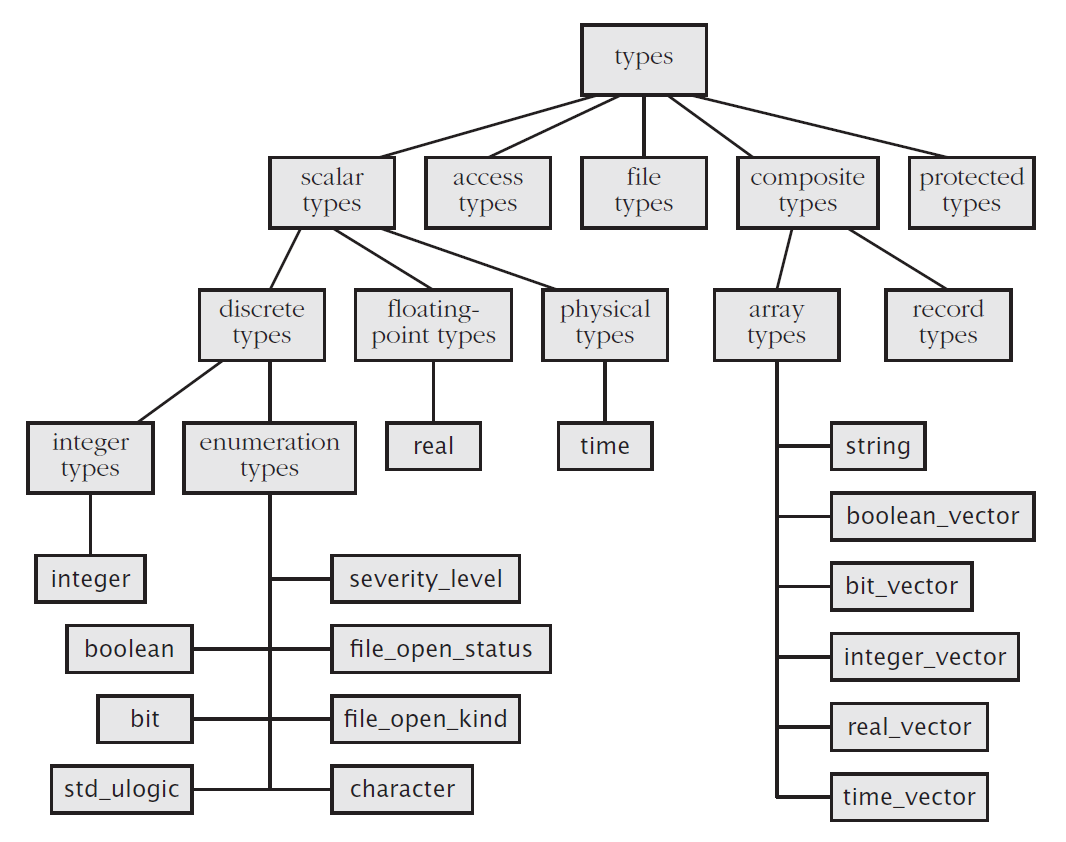
\includegraphics[scale=0.5]{images/TypeHierarchie.png}
    \caption{VHDL Typ Klassifikation}
	\label{TypeHierarchie}
\end{figure}

\subsection{\textit{Integer}}
Die skalaren \textit{Integer}-Datentypen werden in den JVM-Typ \textit{int} umgewandelt, da der Standard fordert, dass diese mindestens 32-Bit breit sein m�ssen.
Sie werden mit dem linkesten Werte ihres Wertebereichs initialisiert und bei Zuweisungen kann eine Laufzeit�berpr�fung notwending sein.

\lstset{caption={Variablendeklaration mit einem \textit{integer} Typ}, label=datatype_integer_vhdl, numbers=left, language=VHDL}
\lstinputlisting{src/backend/datatype_integer.vhd}

In diesem Beispiel \ref{datatype_integer_vhdl} wird eine Variable \textit{x} mit einem Integer-Subtype mit einem Wertebereich von f�nf bis zehn deklariert.
\lstset{caption={Erzeugter JVM Code}, label=datatype_integer_java, language=Java}
\lstinputlisting{src/backend/datatype_integer.java}

Der aus \ref{datatype_integer_vhdl} erzeugte Code in \ref{datatype_integer_java} enth�lt als erstes die Initialisierung von \textit{x} mit f�nf.
Bei der Zuweisung muss eine Laufzeit�berpr�fung durchgef�hrt werden, ob der neue Wert in dem Wertebereich zwischen f�nf und zehn liegt. Dies geschieht mit Hilfe der Runtime Funktion \textit{checkIsInRange}.
Schl�gt diese �berpr�fung fehl, wird eine Ausnahme geworfen.

Der Datentyp \textit{real} wird gleich behandelt nur mit dem Unterschied, dass nat�rlich der JVM-Typ \textit{float} verwendet wird.
\subsection{Enumerationen}
Der Aufz�hlungs-Typ \todo{text}

\lstset{caption={VHDL Aufz�hlungstyp Deklaration}, label=datatype_enum_vhdl, numbers=left, language=VHDL}
\lstinputlisting{src/backend/datatype_enum.vhd}

\lstset{caption={�quivalenter JVM Code}, label=datatype_enum_java, language=Java}
\lstinputlisting{src/backend/datatype_enum.java}


\lstset{caption={Verwendung des Typs}, label=datatype_enum_usage_vhdl, numbers=left, language=VHDL}
\lstinputlisting{src/backend/datatype_enum_usage.vhd}

\lstset{caption={�quivalenter JVM Code}, label=datatype_enum_usage_java, language=Java}
\lstinputlisting{src/backend/datatype_enum_usage.java}

\subsection{\textit{Records}}
Da \textit{VHDL-Records} zusammengesetzte Datentypen sind, werden diese in eigene Klassen �bersetzt, wobei es f�r jeden \textit{record} eine Klasse erzeugt wird.

\begin{minipage}{.30\textwidth}
	\lstset{caption={\textit{Record}-Deklaration}, label=datatype_record_vhdl, numbers=left, language=VHDL}
	\lstinputlisting{src/backend/datatype_record.vhd}
\end{minipage}
\hfill
\begin{minipage}{.65\textwidth}
	\lstset{caption={Erzeugte Klasse}, label=datatype_record_java, language=Java}
	\lstinputlisting{src/backend/datatype_record.java}
\end{minipage}

F�r den Typ \textit{rec} wird die gleichnamige Klasse generiert. Diese hat einen leeren Konstruktur und einen mit dem alle Felder gesetzt werden.
Zus�tzlich wird die \textit{equlas} Methode �berschrieben, damit die Vergleichsoperatoren auf Instanzen der Klasse anwendbar sind. In dieser Methode werden der Reihe nach alle Felder miteinander verglichen.
In \textit{toString} wird eine Text-Repr�sentation der Werte der Felder zur�ckgegben.

\section{\textit{Foreign Subprograms}}
\textit{Foreign Subprograms} sind Prozeduren und Funktionen die in einer anderen Sprache implementiert sind und vom VHDL Code aus aufgerufen werden, um z.B. C-Code innerhalb von Simulationen verwenden zu k�nnen. Aufgrund der Tatsache das die JVM als Ziel gew�hlt wurde, ergibt sich ein einzigartiger Vorteil.  
Viel von dem f�r die virtuelle Maschine geschriebenen Code kann relativ einfach wieder verwendet werden, in dem nur die entsprechenden Deklarationen geschrieben werden. Die n�chsten zwei Beispiel verdeutlichen dies.

\subsection*{Aufruf einer C-Funktion}
\todo{text}
\lstset{caption={Beispiel f�r einfaches \textit{foreign subprogram}}, label=foreign_sin, language=VHDL}
\lstinputlisting{src/backend/foreign_sin.vhd}

Bei einer Attribute-Deklaration k�nnen bis zu drei Parameter angeben werden, wobei die letzen zwei optional sind:
\begin{itemize*}
\item Der volle Pfad zu der Klasse mit der Implementierung.
\item Der Name der Funktion die aufgerufen werden soll.
\item Die Signatur der Funktion.
\end{itemize*}
Wird der Name und die Signatur nicht angeben, werden sie vom Compiler aus der Deklaration der Prozedur ode Funktion berechnet.

\subsection*{Wiederverwendung von JVM Code}
In \ref{foreign_sin} wir eine Sinus-Funktion deklariert mit einem \textit{real} Parameter. In der zweiten Zeile wird diese Funktion durch das Attribute \textit{foreign} als \textit{foreign subprogram} markiert, wobei der ganze JVM Klassenpfad der Implementierung der Funktion als Parameter angegben wird.
Wird diese Funktion dann sp�ter aufgerufen wird vom Compiler Code erzeugt um \textit{java.lang.Math.sin} aufzurufen.

\lstset{caption={\textit{Foreign Subprogram}, dass einen Swing Dialog �ffnet}, label=foreign_showMessage, language=VHDL}
\lstinputlisting{src/backend/foreign_showMessage.vhd}

Das zweite, komplexere Beispiel in \ref{foreign_showMessage} verdeutlicht wie bei der Attribute-Deklaration neben der Klasse auch der Name \textit{showMessageDialog} der aufzurufenden Prozedur spezifiziert wird.
Als dritte Wert des Attributes wird die Signature der Prozedur angegben.

Wird diese Prozedur \textit{showMessage} aufgerufen, �ffnet sich ein ein Java Swing Fenster und gibt den Text in \textit{msg} aus.
%\chapter{Ausblick}
Diese Arbeit pr�sentiert das Grundlegende Design und die Implemtierung f�r einen VHDL Compiler.
Allerdings bietet dieser noch eine Reihe von M�glichkeit wie er erweitert werden kann:
\begin{itemize}
\item die in \ref{Leistungsumfang} erw�hnten Einschr�nken sollten komplett unterst�tzt werden
\item VHDL 2008 bietet viele n�tzliche und interessante Eigenschaften die aber teilweise aufwendig zu implementieren sind (z.B. generische Funktionen)
\item die JVM erhiet mit der Version 7 sogenannte "Method Handles" mit denen sich Funktionszeiger modellieren lassen. Es kann untersucht werden, inwiefern dies verwendet werden k�nnen.
\item alternative Back-Ends wie z.B eines f�r LLVM
\end{itemize}
\cleardoublepage
\phantomsection
\chapter*{Danksagung}
\chaptermark{Danksagung}
\addcontentsline{toc}{chapter}{Danksagung}
Als erstes und vor allem m�chte ich mich bei meinem Betreuer Prof. Hanspeter M�ssenb�ck, 
f�r die Betreuung und Unterst�tzung w�hrend dieser Arbeit bedanken. 

Auch geb�hrt meine Eltern Dank, die mein Studium erst erm�glichten und meinen Schwestern 
Sabine und Susanne, f�r deren Unterst�tzungen in jeglicher Hinsicht w�hrend der Dauer der Masterarbeit 
und des Studium und insbesondere f�r das Korrekturlesen dieser Arbeit.

Weiterhin m�chte ich mich bei meinen Freunden und Studienkollegen bedanken, die mich mit zahlreichen 
fachlichen Diskussionen, Ratschl�gen und Hilfestellungen bei Problemen unterst�tzten.
\cleardoublepage
\phantomsection
\addcontentsline{toc}{chapter}{\bibname}
\begin{thebibliography}{12}

\bibitem{ash}
	Ashenden Peter J.
	{\em The Designer's Guide to VHDL}. 
	Morgan Kaufmann Publishers, San Francisco 2002
\bibitem{ieee}
	IEEE: Standard VHDL Language Reference Manual
	{\em IEEE Std 1076-2002}
\bibitem{od}
	Odersky Martin, Spoon Lex, Venners Bill
	{\em Programming in Scala}
\bibitem{par}
	Parr Terence
	{\em The Definitive ANTLR Reference: Building Domain-Specific Languages}
	The Pragmatic Programmers, LLC, Raleigh, NC, and Dallas, TX 2007.
\bibitem{jls}
	Gosling, James, Bill Joy, and Guy Steele, and Gilad Bracha
	{\em The Java Language Specification, Third Edition}
	Addison-Wesley, Boston, 2005. ISBN: 0321246780.
\bibitem{ghdl}
	 http://ghdl.free.fr/
\bibitem{wirth}
	Wirth, Niklaus
	{\em What Can We Do about the Unnecessary Diversity of Notation for Syntactic Definitions?}
	Communications of the ACM, November 1977
\bibitem{moess}
	M�ssenb�ck, Hanspeter
	{\em The Compiler Generator Coco/R, User Manual}
\end{thebibliography}
\chaptermark{\bibname}
%Abbildungsverzeichnis
\cleardoublepage
\phantomsection
\addcontentsline{toc}{chapter}{\listfigurename}
\listoffigures
\chaptermark{\listfigurename}
%Tabellenverzeichnis
%\cleardoublepage
%\phantomsection
%\addcontentsline{toc}{section}{\listtablename}
%\listoftables
%\chaptermark{\listtablename}

%Quellcodeverzeichnis
\cleardoublepage
\phantomsection
\addcontentsline{toc}{chapter}{\lstlistlistingname}
\lstlistoflistings
\chaptermark{\lstlistlistingname}
%Lebenslauf
\cleardoublepage
\phantomsection
%\chapter*{Lebenslauf}
%\chaptermark{Lebenslauf}
\addcontentsline{toc}{chapter}{Lebenslauf}
\includepdf{Lebenslauf} %Lebenslauf einf�gen
%Eidesstattliche Erkl�rung
\cleardoublepage
\phantomsection
\chapter*{Eidesstattliche Erkl�rung}
\chaptermark{Eidesstattliche Erkl�rung}
\addcontentsline{toc}{chapter}{Eidesstattliche Erkl�rung}
Ich erkl�re an Eides statt, dass ich die vorliegende Masterarbeit selbstst�ndig und ohne fremde Hilfe verfasst, andere als die angegebenen Quellen und Hilfsmittel nicht benutzt bzw. die w�rtlich oder sinngem�� entnommenen Stellen als solche kenntlich gemacht habe. Die vorliegende Masterarbeit ist mit dem elektronisch �bermittelten Textdokument identisch.
 
Des weiteren versichere ich, dass ich diese Masterarbeit weder im In- noch im Ausland in irgendeiner 
Form als Pr�fungsarbeit vorgelegt habe.
\vspace{3 cm}
\begin{center}Linz, \monthname{} 2012 \hspace{3 cm} Christian Reisinger, Bakk. techn.\end{center}
\end{document}

%\section{Kapitel} 1
%\subsection{Unterkapitel} 1.1
%\subsubsection{Unterunterkapitel} 1.1.1
%\paragraph{Abschnitt} keine Numerierung kein Inhaltsverzeichniseintrag
%\subparagraph{Unterabschnitt} keine Numerierung kein Inhaltsverzeichniseintrag
%Anhang
%\begin{appendix}
%\section{Beispiel}
%\end{appendix}
%\footnote{1906 -- 1975}
%\todo{Add details.}
%Listings examples
%\lstinline[<Optionen>]{hier kommt der Quellcode...}
%\lstset{language=<Sprache>}
%\begin{lstlisting}[<Optionen>]
%hier kommt dann der Quellcode...
%\end{lstlisting}